%======================================================================
\subsection{BW-SIM-04 --- Built, 1 Nov: rotor stress, hoop-stress contours, sections, export and a script API}\label{sec:sim-rotor-built}
%======================================================================

Requested by the Vector Jet session (VL-P01 turbojet): centrifugal analysis of rotating wheels in the native study
engine. Three commits: the engine and the validation case (\code{e592bd10}), the study-panel additions (\code{74e18fa3}),
and this record with its API note. The logic is one module, \file{src/Mod/BruceWorx/bruceworx\_sim\_post.py}, with no
GUI in it, so the planned simulation workspace (chapter~\ref{sec:sim07-plan}) can call the same functions as the
existing Study panel and as a design script in \code{FreeCADCmd}. The panel changes are thin.

\begin{figure}[!htbp]
\centering
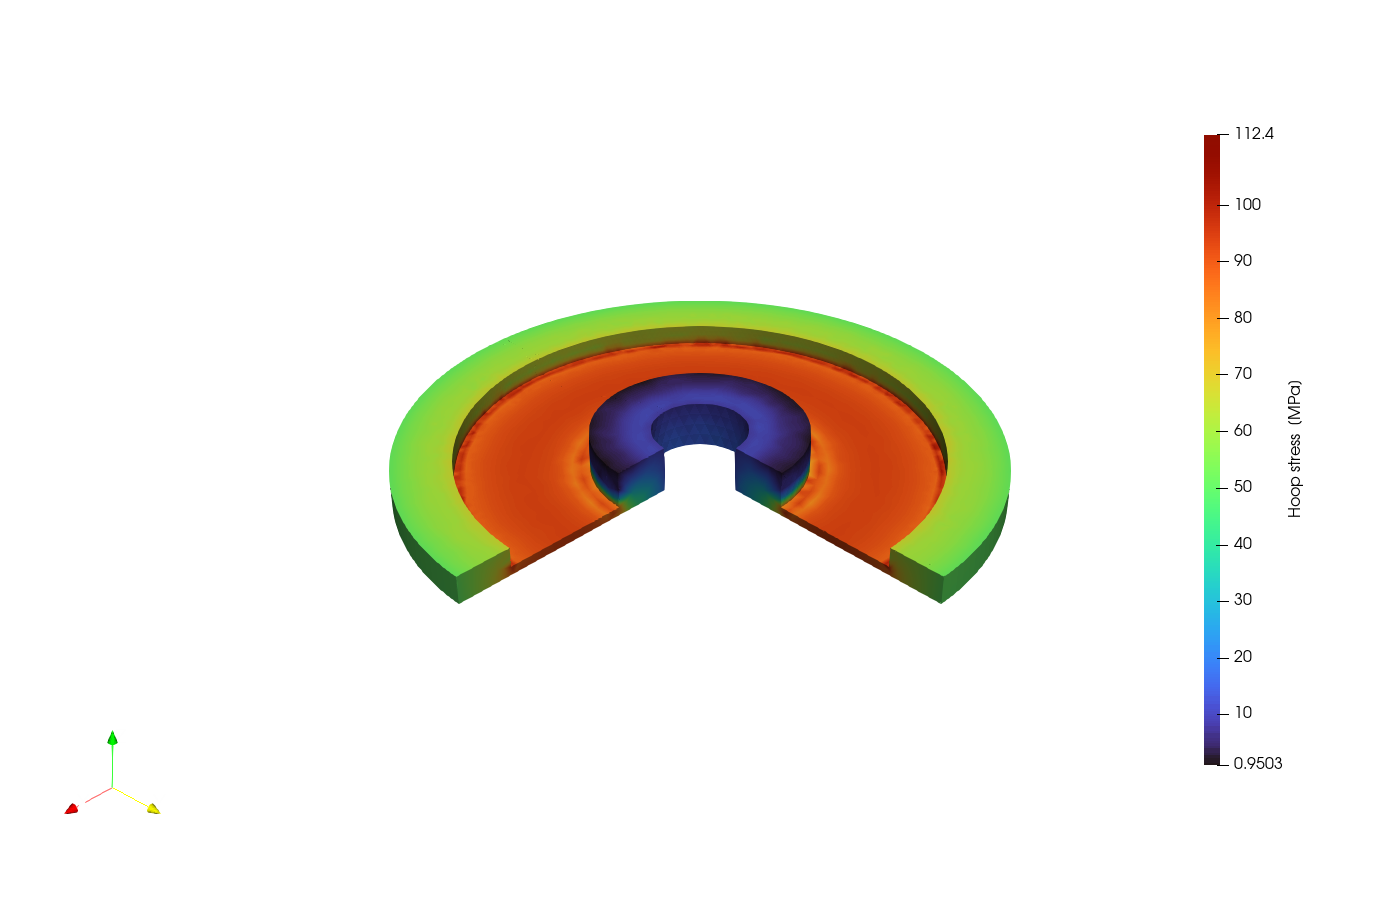
\includegraphics[width=0.49\linewidth]{fig/simrotor_hoop_quarter.png}\hfill
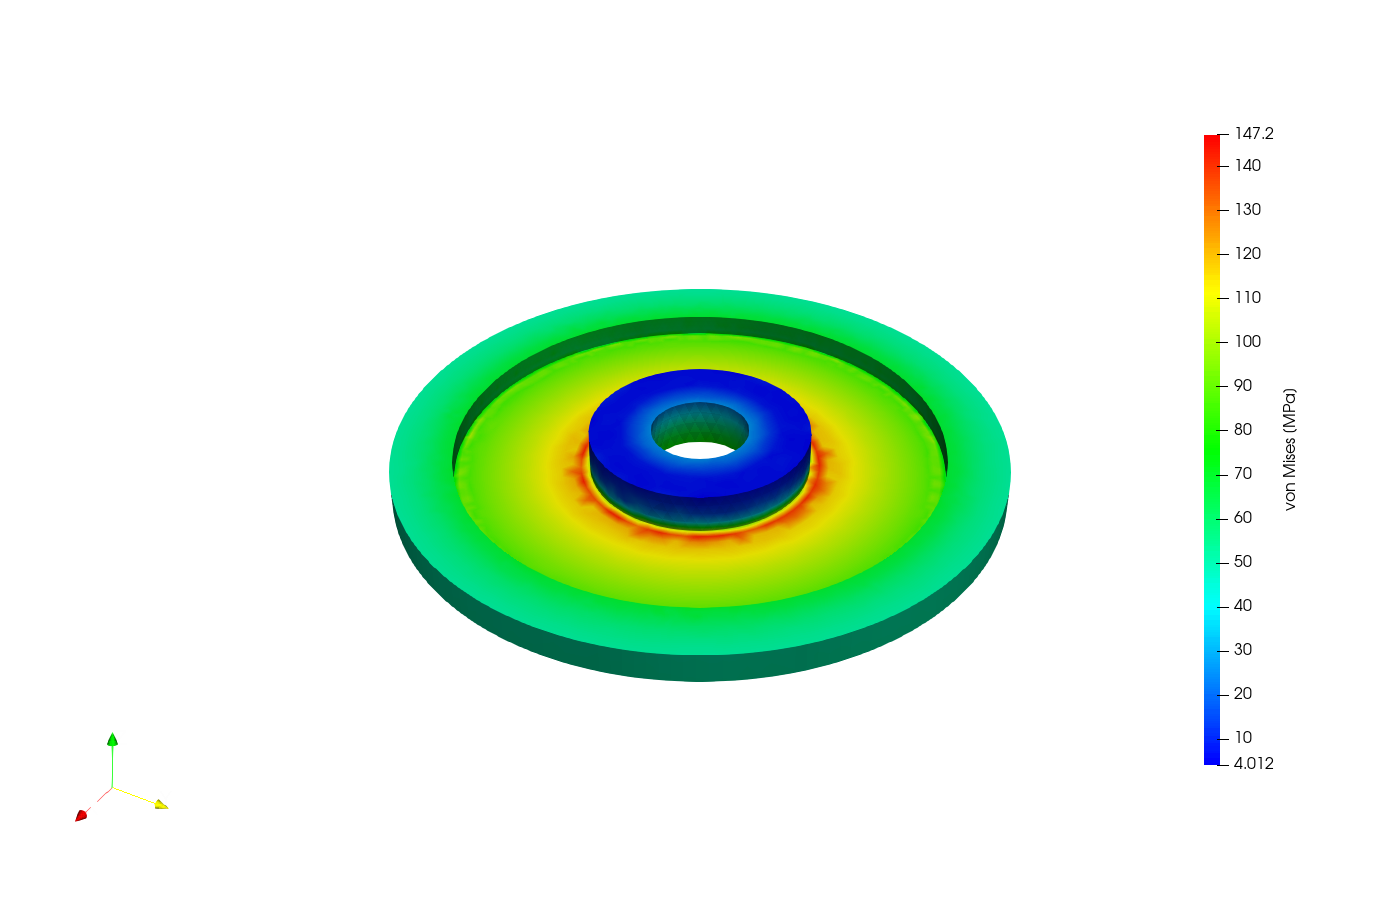
\includegraphics[width=0.49\linewidth]{fig/simrotor_vonmises_iso.png}
\caption{A steel wheel (bore 8, hub, 3\,mm web, rim to $R=50$\,mm; clamped to the shaft in $x$ and $y$, symmetric about
its mid-plane) at 30\,000\,rpm, 7\,481 elements, solved in 1.5\,s. Left: \code{post.contour\_png(an, "hoop",
view="quarter", cmap="turbo")}, a quarter cut away about the spin axis; the web carries 85--95\,MPa of hoop stress, the
rim 55, and the hub, held by the shaft, almost none. Right: von Mises (147\,MPa at the web root), isometric, Rainbow.
Both are off-screen renders by \code{pvbatch} in \code{FreeCADCmd}, no window.}
\label{fig:sim-rotor}
\end{figure}

\paragraph{What you can do now.}
\begin{itemize}[nosep]
  \item \textbf{A spin load.} \code{post.add\_spin(analysis, rpm, axis)} adds FEM's own \code{Fem::ConstraintCentrif}.
        The axis is a circular edge or cylindrical face (its axis), a straight edge, \code{((x,y,z),(dx,dy,dz))}, or
        \code{"x"/"y"/"z"}; with none given it takes the model's largest circle or cylinder. The speed is stored as FEM's
        \code{RotationFrequency} (rpm/60 in 1/s), the label reads ``Spin 30000 rpm'', and the study counts it as a load
        (the members list says ``on the whole model''). The CalculiX input carries the right card: for 30\,000\,rpm,
        \code{Spin,CENTRIF,9869604.4,0,0,-42.4,0,0,1}, $\omega^2=9.8696\times10^6$\,s$^{-2}$ about $+Z$.
  \item \textbf{In the Study panel and the ribbon.} A \textbf{+~Spin} button beside Fixed / Force / Pressure /
        Displacement asks for the speed (default 10\,000\,rpm) and takes the axis from the selected edge or face, else the
        model's bore or rim; the same command is in the ribbon's Setup group.
  \item \textbf{Rim traction needs no new code.} A \emph{Pressure} with \emph{Reversed} on the rim is an outward traction:
        a quarter annulus ($a=10$, $b=50$\,mm) with 10\,MPa reversed on the rim gives $\sigma_\theta(b)$ within 3\,\% of
        Lam\'e's $T(b^2+a^2)/(b^2-a^2)=10.83$ and $\sigma_r=+10$ (tension) at the rim (test).
  \item \textbf{Pre-check.} A spin-only rotor held by a face, symmetry planes or a 3-2-1 on vertices passes (tests for the
        first and the last). It warns when the spin axis misses the part's centre of mass by more than 5\,\% of its size
        (an unbalanced rotor: the supports carry the net centrifugal force), errors when there is no density, and warns
        that point supports pin the rotor's growth locally (read the stress away from them). A spin with no support still
        gets the usual ``No support'' error.
  \item \textbf{Cylindrical stress.} \code{post.cylindrical\_stress(result, axis)} turns the CalculiX nodal tensor into
        radial $\sigma_{rr}$, hoop $\sigma_{\theta\theta}$, axial $\sigma_{zz}$ and shear $\sigma_{r\theta}$ about the spin
        axis (else a picked axis, else the model's). They are stored on the result as \code{StressRadial},
        \code{StressHoop}, \code{StressAxial}, \code{StressRTheta} with the axis, and recomputed only when it changes. The
        panel has Radial, Hoop, Axial and Shear buttons next to Stress, Displacement and Safety Factor, a ``Pick axis''
        button (selected circular edge or cylindrical face) and a ``Spin axis'' button to go back; the ribbon has a Hoop
        Stress command.
  \item \textbf{Colour map, range, section.} Rainbow (the current look), Turbo and Jet; a fixed colour range per study and
        field (the boxes and the Fixed tick in the panel, stored as \code{RangeFixed\_hoop}, \code{RangeMin\_hoop},
        \code{RangeMax\_hoop} on the study); a half or quarter \textbf{Section} about the axis. Von Mises and displacement
        keep FEM's own colouring until the study asks for another map, range or section.
  \item \textbf{Export.} \code{post.export\_vtu} writes the result with the displacement, the stress tensor, von Mises, the
        principal stresses, the safety factor and \code{Radial}, \code{Hoop}, \code{Axial}, \code{RTheta}, the axis as field
        data, quadratic tetrahedra kept as such. The panel has \textbf{Export .vtu}, \textbf{ParaView} (writes a view script
        with the shown field, the study's colour map, range and section, and starts the app through
        \code{bruceworx\_cfd\_paraview.paraview\_executables}) and \textbf{Picture} (PNG from the 3D view).
  \item \textbf{Scripts.} The whole flow runs in \code{FreeCADCmd}: \code{new\_study}, \code{add\_spin}, \code{mesh\_study},
        \code{solve}, \code{contour\_png}, \code{radial\_plot}, \code{export\_vtu}. \file{SCRATCH/agent-rotor/API.md} has the
        exact calls for the Vector Jet design scripts.
\end{itemize}

\paragraph{Validation, case G-RD1 (closed form, tier G).} A thin steel annulus ($a=10$, $b=50$, 2\,mm thick, a quarter with
symmetry planes) at 30\,000\,rpm against Timoshenko and Goodier's plane-stress disc,
$\sigma_\theta(a)=\tfrac14\rho\omega^2[(3+\nu)b^2+(1-\nu)a^2]=161.15$\,MPa. Bore and rim are the mean of the nodes on the
circle; mid-radius ($r=30$) is a cubic fit over the radius on the mid-plane. Tolerance 3\,\%, every row passes on both
sets:
\begin{center}
\small
\begin{tabular}{@{}lrrrr@{}}
\toprule
 & closed form & fast (4\,mm, 8\,821 nodes) & slow (3\,mm, 9\,580 nodes) & error (3\,mm)\\
\midrule
hoop at the bore $r=10$ & 161.151 & 161.136 & 161.140 & $-0.007$\,\%\\
hoop at the rim $r=50$ & 40.288 & 40.288 & 40.288 & $+0.001$\,\%\\
radial at $r=30$ & 45.453 & 45.739 & 45.732 & $+0.62$\,\%\\
hoop at $r=30$ & 75.410 & 75.153 & 75.157 & $-0.34$\,\%\\
\bottomrule
\end{tabular}
\end{center}
The closed form itself is checked in \file{TestBruceWorxValidation} (free at both radii, the bore formula, the solid disc's
centre) and the numbers in \file{cases.json} are regenerated from it.

\paragraph{Decided while building.}
\begin{itemize}[nosep]
  \item \textbf{FEM wants a line.} The CalculiX writer for \code{ConstraintCentrif} reads the first \emph{straight} edge of
        its axis reference and, for anything else (a circle, a face), silently falls back to the global Z axis through the
        origin. So \code{add\_spin} resolves the pick to point and direction and makes a hidden \code{Part::Line}
        (\code{SpinAxis}) for FEM; a wheel on any axis spins about the right one.
  \item \textbf{Cylindrical components are ours, from the tensor.} FEM's result object has only Cartesian stress, so the
        components are computed per node from \code{NodeStressXX..YZ} and the node positions (numpy, no FreeCAD in the
        maths; tested on an axisymmetric field, a tilted axis and the axis itself, where radial and hoop have no
        direction and both take the mean in-plane normal stress).
  \item \textbf{The GUI paints with its own colour map.} FEM's mesh view only has its built-in scale, so Turbo, Jet, a
        fixed range and the section go through \code{NodeColor} (64 colours of the map, grouped by node); the legend is a row
        of chips. Von Mises and displacement stay on FEM's scalar colouring while nothing else is asked, so existing
        studies look as before.
  \item \textbf{The panel's section is element-wise.} It makes a mesh object (outside the study) of the elements whose centre
        is not in the removed quadrant, so the cut is jagged by one element; the pictures cut exactly (a plane clip in
        ParaView). I did not use FEM's post clip filter in the panel because it cannot carry our colour maps. A quarter model has nothing left after a
        quarter cut, so that is refused with the reason (the first GUI run crashed on an empty section mesh).
  \item \textbf{Pictures are pvbatch.} \code{contour\_png} always exports the .vtu and draws it with ParaView's \code{pvbatch}
        (the same colour table sampled from the map, so GUI and picture agree), also when called inside the GUI. Without
        ParaView it raises a \code{PostError} with the install hint instead of hanging. The panel's \textbf{Picture} uses
        the 3D view, as the report's renders do.
  \item \textbf{A balanced rotor needs no particular support.} The net centrifugal force is zero, so a face on the bore, symmetry
        planes or a 3-2-1 all work; but a point support pins the growth there (a stress spike at the pin), which is why the
        validation model uses symmetry planes and the pre-check warns about points.
\end{itemize}

\paragraph{Tests.} Headless \file{TestBruceWorxSimRotor.py} (21, 0 failures): the cylindrical components on an axisymmetric
field, a tilted axis and the axis itself; colour maps; the closed form; axis from a cylinder face and a circle edge (and a
plane refused); \code{add\_spin} (the rpm $\leftrightarrow$ frequency round trip, label, a load of the study, a speed change,
zero refused); the model's own axis; the pre-check (balanced and held by a face, 3-2-1 with its warning, an axis that misses
the part, no density, no support, ranges and colour map stored); one solve of the G-RD1 annulus read by six tests (the
\code{*DLOAD} card at $\omega^2$ with axis $+Z$, the closed-form stress, the stored components and their trace, the .vtu with
every field and quadratic cells, the radial profile against the closed form within 4\,\%, a \code{pvbatch} picture); and the
reversed-pressure rim traction against Lam\'e. \file{TestBruceWorxValidation} and \file{TestBruceWorxSimCore} with them: 105
tests, 0 failures. GUI, \file{TestBruceWorxSimulation} (14), \file{TestBruceWorxWorkspaces} (25), \file{TestBruceWorxValidationGui}
(1), 0 failures; the new GUI test covers the + Spin button, the four fields, Turbo, the fixed range, the quarter section of a
whole wheel (75\,\% of the elements stay), the refused section, a picked axis and the spin axis again, the .vtu, the ParaView
script and a picture.

\paragraph{Open questions for you.}
\begin{enumerate}[nosep]
  \item \textbf{The section in the panel} is jagged by one element (it leaves whole elements out). A smooth cut means FEM's
        post pipeline, which has its own colour scale (Rainbow only) and no fixed-range or Turbo option. Keep ours, or accept
        FEM's colours for the sectioned view?
  \item \textbf{A rotor support helper.} A full wheel with no symmetry needs the user to add a bore or hub constraint. Offer
        a ``Hold bore'' button that adds a Fixed constraint on the selected cylindrical face (stiffer than a real shrink fit),
        or a radial-free support (a cylindrical \code{ConstraintTransform}, not built)?
  \item \textbf{Blade pull and thermal.} Blade centrifugal pull is a Pressure on the rim today (the user computes it).
        Should a ``Blade mass'' load do it from the blade count, mass and radius, and should the spin combine with a thermal
        study (hot disc, thermal stress plus centrifugal)? Today the spin load is checked and solved in static studies only.
  \item \textbf{Burst margin.} Report a burst speed ($\sqrt{\text{UTS}/\sigma_{\text{avg hoop}}}$, ``Zwicky'' style) beside the
        safety factor?
\end{enumerate}

\paragraph{Your answers (1 Nov).} (1) Keep our section for now. (2) Built as \code{hold\_for\_spin} in the review rounds
below. (3) Yes: a \emph{Blade mass} load from the blade count, mass and radius, and spin combined with a thermal study.
(4) Yes: report the burst speed beside the safety factor. A tilted-axis \code{hold\_for\_spin} stays for later.


\subsection*{Follow-up: review by the Vector Jet session}

The Vector Jet session cross-checked the rotor stress on a real turbine disc (hoop and radial stress agree with its own
reading to 0.0000\,MPa on 26\,776 nodes) and found six things; all are fixed and tested.

\begin{enumerate}[nosep]
  \item \textbf{Wrong support advice.} A Fixed face on the bore stops the bore growing and kills the bore hoop stress. The
        how-to, the pre-check and the panel now say: axial-only on a flat face plus a minimal 3-2-1 point set, or symmetry
        planes on a sector. A Fixed (or radially fixing Displacement) on a cylindrical face coaxial with a spin axis is a
        pre-check \emph{error} with that explanation. The helper you were asked about is built:
        \code{post.hold\_for\_spin(analysis, face=...)} and a \emph{+ Hold for spin} button add the axial-only face, point A
        (the vertex nearest the axis, both directions across it) and point B (the vertex with the longest lever arm, one
        direction). The axis must lie along X, Y or Z. Test: a full thin wheel with no symmetry planes, held by the helper,
        gives the Timoshenko bore hoop within 8\,\%.
  \item \textbf{Bore reporting.} The mean hoop over the bore is right for a thin disc only (a 14\,mm hub: mean 340, mid-plane
        404, von Mises 512\,MPa). \code{post.bore\_stress(result, analysis)} gives hoop mean, max and mid-plane, von Mises
        max and mid-plane and the lowest safety factor on the bore; the summary, the panel and the report show them. The
        safety factor divides the study's equivalent stress (von Mises by default), never the hoop stress; the report says so.
  \item \textbf{\code{working\_dir}.} FEM fell back to a temporary folder when the given one did not exist yet;
        \code{prepare\_solve} now creates it. Tested with a nested missing folder.
  \item \textbf{Faceted pictures.} \code{contour\_png} sets \code{NonlinearSubdivisionLevel = 2}, so quadratic tetrahedra are
        curved, and hides ParaView's orientation triad (\code{axes=True} brings it back).
  \item \textbf{Mesh failures.} \code{mesh\_study} raises a clear error for a mesh with no volume elements; when second order
        was asked and Netgen returned linear tetrahedra it upgrades them to Tet10 with straight mid-edge nodes (FEM order
        1-2, 2-3, 3-1, 1-4, 2-4, 3-4, checked against Netgen's own) and says so; an upgraded mesh solves to the closed form.
  \item \textbf{Unused nodes and singular solves.} A failed second-order step left about 135\,000 nodes that no element uses;
        a nearest-node support could land on one and ccx returned $10^9$\,MPa without an error. \code{mesh\_study} now drops
        nodes no element uses, and a static solve whose largest displacement exceeds $10^3$ times the model size raises
        ``unsupported or singular''. The 1\,GB impeller STEP itself was not re-run; the cases are synthetic.
\end{enumerate}

\paragraph{Tests.} \file{TestBruceWorxSimRotor} now has 35 tests (was 21): the fixed-bore error (Fixed and Displacement), the
axial-only bore face accepted, \code{hold\_for\_spin}, the full held wheel, \code{bore\_stress}, \code{working\_dir}, the
surface-only, unused-node and Tet10 upgrade cases, the singular guard and the picture script.

\paragraph{Second round of the same review.}
\begin{enumerate}[nosep]
  \item \textbf{The support set is now a pure vertex 3-2-1.} Point B holds a direction that is \emph{tangential} at B (it
        picks the largest radius whose tangent is the global X, Y or Z, so a vertex on the $+X$ radius holds Y; a warning
        names the tangential share when no vertex has such a tangent). A holds both directions across the axis, C (a vertex
        off the line A--B) holds the axial direction; A and B hold it too, so the three axial points fix the two tilts. A
        flat face is used only when you pick one. A plain annulus has every vertex on its seam, so there is no C: the axial
        direction is held along a circular edge at A's level instead (a balanced rotor's axial shift is the same all round the
        edge, so it costs no stress). \emph{What the 8\,\% was:} only the bound of the earlier test. Measured on the whole 2\,mm
        annulus with no symmetry planes, the bore hoop was $+0.028\,\%$ with the face-based set (size 5) and $+0.089\,\%$ on a
        4\,mm disc (size 6); with the point set it is $+0.027\,\%$ (size 5) and $+0.006\,\%$ (size 3). The earlier B was already
        tangential on the annulus (it sits on the seam), but could have been partly radial elsewhere; the axial face held back
        the Poisson thinning a little (the 4\,mm case). Validation case \textbf{G-RD2} (whole annulus, tolerance 0.2\,\%) and
        tests for the annulus, a sector with a true vertex 3-2-1, and the face option.
  \item \textbf{Elements not connected through faces.} After the Tet10 upgrade and the removal of unused nodes, Netgen could
        still leave a few elements that touch the wheel only at a node or an edge: a mechanism. \code{mesh\_study} now keeps the
        largest body connected through shared faces (union-find over each face's sorted corner nodes) and drops the rest; the
        count and the number of clusters are in \code{stats["notes"]} and the progress text. Tested with a tet hanging by one
        node and one hanging by an edge.
\end{enumerate}

\paragraph{Third round (the real bladed impeller).}
\begin{enumerate}[nosep]
  \item \textbf{\code{bore\_stress} found the wrong bore} (radius 4.913, $z_{\mathrm{mid}}$ 67.97, 36 nodes on a bore of
        $r=5$ from $z=-3$ to $23.5$). Two causes. The bore was ``the nodes within 0.1\,\% of the smallest radius'': those are
        the straight mid-edge nodes of the quadratic tetrahedra, which sit a little \emph{inside} the true radius
        ($5\cdot(1-\cos(\theta/2))\approx0.09$\,mm), so only 36 nodes qualified. And $z$ was measured from the axis point, which
        is the start of the hidden \code{SpinAxis} line ($z=-38.2$ on this part), not from the global origin. Now the bore is the
        set of nodes the mesh has \emph{on} the concave cylindrical face(s) coaxial with the spin axis (smallest radius; a
        convex journal is not a bore; \code{bore\_faces}), mid-edge nodes included, and $z$ is the position along the axis
        direction in global coordinates. Test: a bore $r=5$, $z\in[-3,23.5]$ on an axis off the origin.
  \item \textbf{The bore's safety factor was not the part's.} \code{bore\_stress} returned the lowest factor of the bore
        nodes under the key \code{min\_sf} (3.00 on the impeller; the wheel's real minimum is on the back plate). It is now
        \code{bore\_min\_sf}, printed as ``Bore only'' in the panel and the report; the part's factor everywhere
        (\code{result\_extrema}, panel, report) is the minimum over all nodes, labelled ``Min safety factor, whole part''. The
        ``away from the supports'' minimum now also leaves out every node within $2\times$ the element size of a point support
        (a pin has a stress spike round it), and the panel and report say so with the radius.
\end{enumerate}


\paragraph{Follow-up, 1 Nov: blade mass, spin with heat, burst speed.}
Your three answers, built; the tilted-axis \code{hold\_for\_spin} and the section view are as they were.
\begin{itemize}[nosep]
  \item \textbf{Blade mass load.} \code{post.add\_blade\_mass(analysis, faces, count, mass\_g, r\_cg\_mm)} and a \textbf{+~Blade
        mass} button (select the rim face(s); it asks for the count, the mass and the radius). Each blade pulls with
        $F=m\,r_{cg}\,\omega^2$ at the study's spin speed; the total $N F$ is spread \emph{evenly} over the area of the
        selected faces, so the pressure is $N F/A$ (an outward traction: FEM's Pressure with Reversed, nothing new for the
        solver). The blades are not placed at their angles: a real blade root loads its seat unevenly, so this is the
        average pull; for the stress at the seats model them. $N$ is the number of blades the selected faces carry, so a
        sector model takes its share (a quarter of a 24-blade wheel: 6; our validation eighth, a quarter cut at the
        mid-plane: 3, a share of a blade is allowed). The load keeps the blade data on itself and follows the first spin
        load: \code{set\_spin\_speed} refreshes it, and so does every pre-check and solve, so a speed edited in the property
        view cannot leave a stale pull. The pre-check errors without a spin load or with a zero count, mass or radius, and
        warns when a selected face does not face outward from the axis. The study lists it as ``Blade mass 24 x 2 g at
        55 mm: 1085.7 N each, 26056 N over 628.3 mm$^2$''. Example: 24 blades of 2\,g at $r_{cg}=55$\,mm and 30\,000\,rpm
        pull 1085.66\,N each, 41.47\,MPa on the rim of the G-RD1 annulus.
  \item \textbf{Validation case G-RD3.} G-RD1's quarter annulus with that load against the Timoshenko disc plus Lam\'e's
        outer tension (\code{post.rotating\_disc\_rim}), tolerance 3\,\%. On the 3\,mm mesh (9\,580 nodes): bore hoop
        247.545 closed form, 247.527 solved ($-0.007$\,\%); rim hoop 85.213, 85.212 ($0.000$\,\%); radial at $r=30$ 83.850,
        84.273 ($+0.51$\,\%); hoop at $r=30$ 123.407, 123.010 ($-0.32$\,\%). The pull adds 86\,MPa at the bore to the 161.15
        of the plain disc. Unit tests: the closed forms (zero traction is the plain disc, $\sigma_r(b)=T$, $\sigma_r(a)=0$),
        the pressure times the area equals $N F$, the load follows the speed, the errors and the outward warning.
  \item \textbf{Spin with heat.} The spin load, the blade mass and \textbf{+~Hold for spin} are checked and solved in
        thermal stress studies too (before only in static ones; CalculiX's \code{*DLOAD CENTRIF} rides in the same step as the
        temperature, and the panel offers the buttons). Superposition on the quarter annulus (bore 120\,$^\circ$C, rim
        20\,$^\circ$C, $T_{ref}=20$, steady conduction), 3\,mm mesh, hoop stress: bore $-184.15$ (heat only) $+161.14$
        (spin only, a static study) $=-23.01$, combined solve $-23.01$ (difference below 0.001\,MPa); rim $67.79+40.29=108.08$,
        combined $108.08$. Against the closed form (Timoshenko disc plus the thermal disc by quadrature,
        \code{post.thermal\_disc}): bore $-23.06$ ($-0.20$\,\%), rim $108.08$ ($0.00$\,\%).
  \item \textbf{Burst speed.} $n_{burst}=n\sqrt{\mathrm{UTS}/\sigma_{avg}}$, $\sigma_{avg}$ the hoop stress averaged over the
        disc's meridional section: each tetrahedron counts with its volume$/(2\pi r)$ (its section area) and the mean of
        its corner hoop stresses. UTS is the \code{UltimateTensileStrength} of the study's material card, without the
        knockdown, named in the line (``the material card has no ultimate tensile strength'' gives no figure and says so).
        The panel, the summary text and the report print the burst speed and the margin $n_{burst}/n$ beside the safety
        factor; the bore safety factor and the part's are unchanged. G-RD1 annulus at 30\,000\,rpm with UTS 900\,MPa: average
        hoop 80.11\,MPa (the closed form's mean over the radius agrees within 1\,\%), $n_{burst}=100\,554$\,rpm, margin 3.35, while
        the part's safety factor against a 355\,MPa yield is 2.20. The hot disc gives the same 80.12\,MPa: heat stress balances
        over the section, so it hardly moves the average. The estimate assumes the stress grows with $n^2$, which thermal
        stress does not, and uses the card's room temperature UTS; the report says so.
\end{itemize}
\textbf{Tests.} \code{TestBruceWorxSimRotor} 49 (was 35), \code{TestBruceWorxSimCore} 57 and \code{TestBruceWorxValidation} 32, 0
failures. \textbf{Open questions.} (1) Should the blade pull follow the spin automatically when a study has several spin loads
(today the first)? (2) A real blade root loads its seat unevenly; do you want a per-seat pull on a chosen set of faces
later? (3) The burst margin has no pass/fail threshold; add one (many specifications ask for 1.2 or more)?
